\documentclass{article}

\usepackage{graphicx}
\usepackage{tikz}
\usepackage{tikzsymbols}
\usetikzlibrary{calc,patterns,shapes.geometric}
\pagestyle{empty}
\usepackage[margin=0pt]{geometry}
\geometry{papersize={14in,12in}}

\def\centerarc[#1](#2)(#3:#4:#5){\draw[#1] ($(#2)+({#5*cos(#3)},{#5*sin(#3)})$) arc (#3:#4:#5);}

\begin{document}
	\begin{figure}
		\centering
		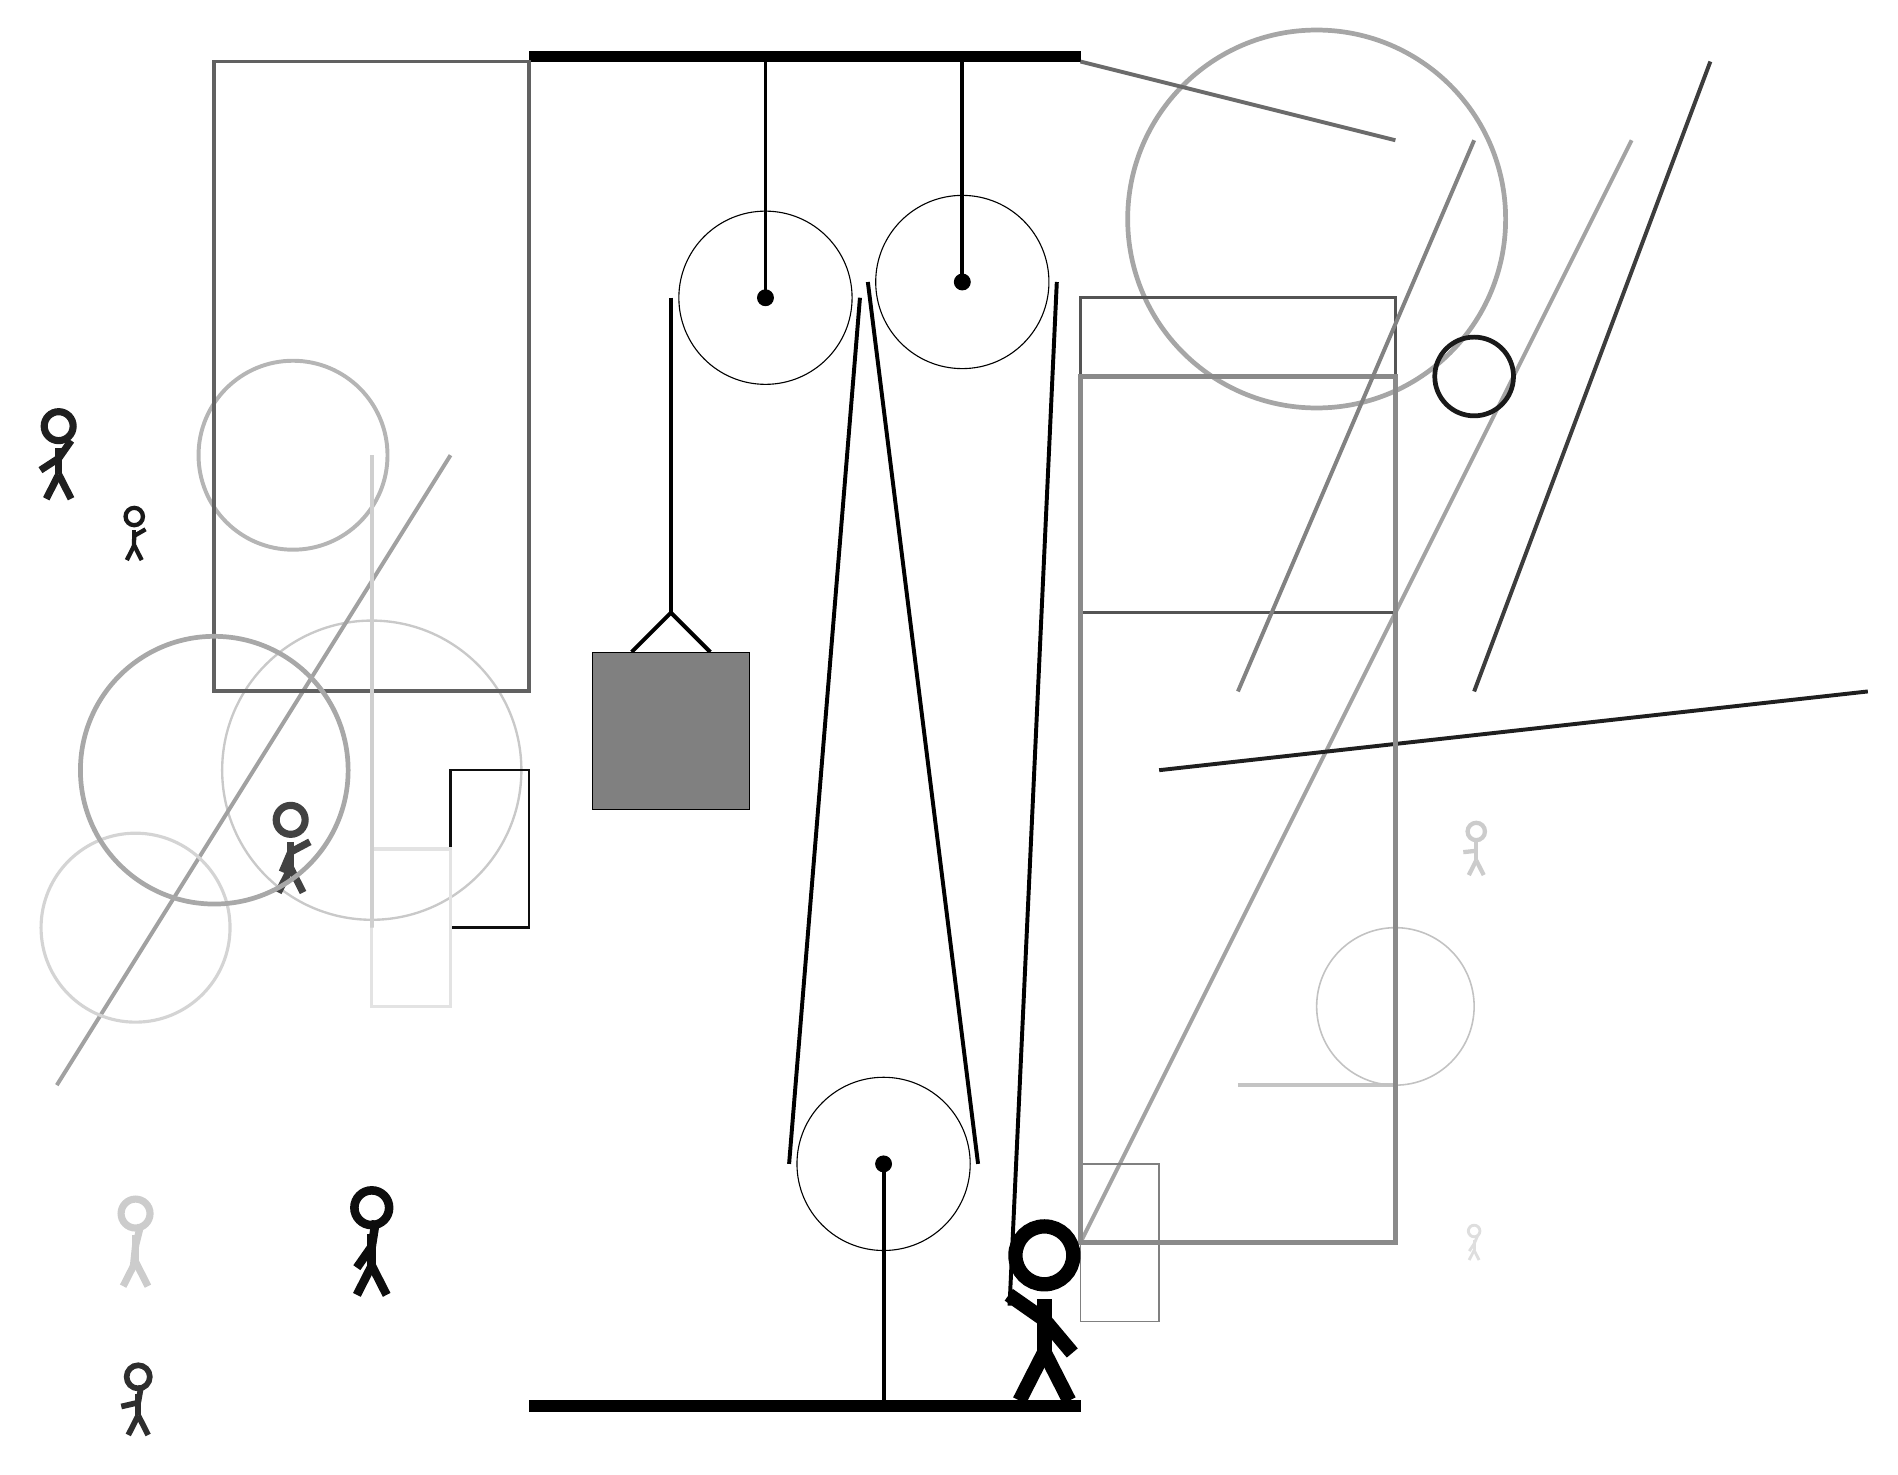
\begin{tikzpicture}
			%%%%% START %%%%%
			
			\draw[fill=black] (-2, 14) rectangle (5, 14.125);
			
			\draw (1, 11) circle (1.1);
			\draw[fill=black] (1, 11) circle (0.1);
			\draw[line width=0.5mm]  (1, 14) -- (1, 11);
			
			\draw[fill=white](2.5, 0) circle (1.1);
			\draw[fill=black] (2.5, 0) circle (0.1);
			\draw[line width=0.5mm]  (2.5, -3) -- (2.5, 0);
			
			\draw[fill=white](3.5, 11.2) circle (1.1);
			\draw[fill=black] (3.5, 11.2) circle (0.1);
			\draw[line width=0.5mm] (3.5, 14) -- (3.5, 11.2);
			
			\draw [line width=0.3mm, color=black!21](-4, 5) circle (1.9);
			
			\draw [line width=0.6mm, color=black!35](8, 12) circle (2.4);
			\node[line width=0.3mm, color=black!20] at (10, 4) {\Strichmaxerl[3][6][90]};
			\node[line width=0.3mm, color=black!74] at (-5, 4) {\Strichmaxerl[5][67][28]};
			\draw[line width=0.5mm, color=black!23](7, 1) -- (9, 1);
			
			\draw[line width=0.5mm, color=black!36](5, -1) -- (12, 13);
			\draw [line width=0.5mm, color=black!29](-5, 9) circle (1.2);
			\draw[line width=0.3mm, color=black!94] (-2, 5) rectangle (-3, 3);
			\draw[line width=0.5mm, color=black!88](6, 5) -- (15, 6);
			\draw[line width=0.5mm, color=black!76](10, 6) -- (13, 14);
			
			\node[line width=0.6mm, color=black!90] at (-7, 8) {\Strichmaxerl[3][88][30]};
			\draw[line width=0.2mm, color=black!50] (6, -2) rectangle (5, 0);
			\node[line width=0.3mm, color=black!82] at (-7, -3) {\Strichmaxerl[4][13][80]};
			
			\draw [line width=0.2mm, color=black!24](9, 2) circle (1.0);
			\draw [line width=0.6mm, color=black!90](10, 10) circle (0.5);
			\draw[line width=0.5mm, color=black!37](-3, 9) -- (-8, 1);
			
			\draw[line width=0.4mm, color=black!67] (5, 7) rectangle (9, 11);
			
			\draw[line width=0.5mm, color=black!58](5, 14) -- (9, 13);
			\draw[line width=0.5mm, color=black!62] (-2, 6) rectangle (-6, 14);
			\draw [line width=0.4mm, color=black!17](-7, 3) circle (1.2);
			\node[line width=0.3mm, color=black!13] at (10, -1) {\Strichmaxerl[2][56][67]};
			
			\node[line width=0.4mm, color=black!20] at (-7, -1) {\Strichmaxerl[5][84][76]};
			\node[line width=0.6mm, color=black!95] at (-4, -1) {\Strichmaxerl[6][55][81]};
			\node[line width=0.4mm, color=black!88] at (-8, 9) {\Strichmaxerl[5][33][55]};
			\draw [line width=0.6mm, color=black!34](-6, 5) circle (1.7);
			
			\draw[line width=0.4mm, color=black!11] (-4, 2) rectangle (-3, 4);
			\draw[line width=0.5mm, color=black!19] (-4, 9) rectangle (-4, 3);
			\draw[line width=0.7mm, color=black!46] (5, -1) rectangle (9, 10);
			
			\draw[line width=0.5mm, color=black!49](10, 13) -- (7, 6);
			
			\draw[line width=0.5mm] (-0.7, 6.5) -- (-0.2, 7.0) -- (0.3, 6.5);
			\draw[fill=black!50] (-1.2, 6.5) rectangle (0.8, 4.5);
			
			\draw[line width=0.5mm] (-0.2, 11) -- (-0.2, 7.0);
			\centerarc[line width=0.5mm](1, 11)(0:180:1.2000000000000002);
			\draw[line width=0.5mm](2.2, 11) -- (1.3, 0);
			\centerarc[line width=0.5mm](2.5, 0)(180:360:1.2000000000000002);
			\draw[line width=0.5mm](3.7, 0) -- (2.3, 11.2);
			\centerarc[line width=0.5mm](3.5, 11.2)(0:180:1.2000000000000002);
			\draw[line width=0.5mm](4.7, 11.2) -- (4.1, -1.8);
			
			\node at (4.5, -1.9) {\Strichmaxerl[10][-35][-50]};
			
			\draw[fill=black] (-2, -3) rectangle (5, -3.15);
			
			%%%%% END %%%%%
		\end{tikzpicture}
	\end{figure}	
\end{document}